\chapter{Supplementary material for Chapter \getrefnumber{ch:Transcriptomics}}

\begin{comment}
\begin{figure}
\centering
\begin{subfigure}[b]{0.60\textwidth}
\centering \includegraphics[width=\textwidth]%
{transcriptomics/UniqueExpression/Castle_1.pdf}
\caption{Castle}\label{fig:UniqueExprCastle}
\end{subfigure}%
~%
\begin{subfigure}[b]{0.60\textwidth}
\centering \includegraphics[width=\textwidth]%
{transcriptomics/UniqueExpression/Brawand_1.pdf}
\caption{Brawand}\label{fig:UniqueExprBrawand}
\end{subfigure}

\begin{subfigure}[b]{0.60\textwidth}
\centering \includegraphics[width=\textwidth]%
{transcriptomics/UniqueExpression/IBM_1.pdf}
\caption{IBM}\label{fig:UniqueExprIBM}
\end{subfigure}%
~%
\begin{subfigure}[b]{0.60\textwidth}
\centering \includegraphics[width=\textwidth]%
{transcriptomics/UniqueExpression/Uhlen_1.pdf}
\caption{Uhlen}\label{fig:UniqueExprUhlen}
\end{subfigure}

\begin{subfigure}[b]{0.95\textwidth}
\includegraphics[width=\textwidth]%
{transcriptomics/UniqueExpression/Gtex_1b.pdf}
\caption{Gtex}\label{fig:UniqueExprGtex}
\end{subfigure}
\caption{Protein coding genes expressed per tissues}
\end{figure}
\end{comment}


\begin{figure}[htpb]
\includegraphics[scale=0.65]{transcriptomics/PcodingGenesExpressed0_4tissues.pdf}\centering
\caption[Unique and shared protein coding genes expressed
in the 4 common tissues]{\label{fig:ExpGenePcoding0_4T}\textbf{Unique and
shared protein coding genes expressed (at any level) in the 4 common tissues.}}
\end{figure}


\begin{table}[]
\centering
\caption[Expressed protein coding genes]{\textbf{Expressed protein coding genes.}\\
{\small In \ens{76}, there are 22,469 genes that
have a biotype annotated as \enquote{\emph{protein coding}}.}}
\label{tab:expGenesPcoding}
\begin{tabular}{@{}cccccccc@{}}
\toprule
\multirow{4}{*}{Dataset} &
\multirow{4}{*}{\begin{tabular}[c]{@{}c@{}}Number of \\ Tissues\end{tabular}} &
\multicolumn{2}{c}{\multirow{2}{*}{\begin{tabular}[c]{@{}c@{}}Number of mRNAs \\
expressed across \\ all tissue\end{tabular}}} &
\multicolumn{4}{c}{Number of mRNAs expressed at least once} \\
\cmidrule(l){5-8}
&  & \multicolumn{2}{c}{} &
\multicolumn{2}{c}{\begin{tabular}[c]{@{}c@{}}4 common\\  tissues\end{tabular}} &
\multicolumn{2}{c}{\begin{tabular}[c]{@{}c@{}}23 common\\  tissues\end{tabular}} \\
\cmidrule(l){3-8}
&  & ›0 FPKM & ≥ 1FPKM & ›0 FPKM & ≥ 1FPKM &
\multicolumn{1}{l}{›0 FPKM} & \multicolumn{1}{l}{≥ 1FPKM} \\
\midrule
Castle & 11 & 19,066 & 15,798 & 18,477 & 13,443 & --- & --- \\
Brawand & 8 & 19,505 & 16,410 & 19,324 & 15,327 & --- & --- \\
IBM & 16 & 19,776 & 17,171 & 19,334 & 15,058 & --- & --- \\
Uhlén & 32 & 19,807 & 18,060 & 19,379 & 15,739 & 19,737 & 17,832 \\
GTEx & 47 & 20,272 & 18,386 & 20,242 & 16,100 & 20,263 & 18,013 \\ \bottomrule
\end{tabular}
\end{table}


\begin{figure}[htpb]
    \includegraphics[scale=0.85]{transcriptomics/heatmap4TWithMitoNoRep_1.pdf}\centering
    \caption[Comparison of profiles across the 5 studies for their
    4 common tissues --- with the 37 mitochondrial genes
    included]{\label{fig:ExpGenePcoding1_withMito}\textbf{Comparison of profiles
    across the 5 studies for their 4 common tissues --- with the 37
    mitochondrial genes.}}
\end{figure}

\begin{figure}[htpb]
    \includegraphics[scale=0.95]{transcriptomics/heatmapT4NoMitoAndwithRep_1.pdf}\centering
    \caption[Heatmap including all the replicates of the 4 common tissues
    across the 5 studies]{\label{fig:noMitoRep4T}\textbf{Heatmap including all
    the replicates of the 4 common tissues across the 5 studies.} All protein
    coding genes (except the mitochondrial ones)
    at least expressed at 1 \FPKM\ are included. All the samples, except from the
    \castle\ study are clustering by their tissue of origin.
    Remarkably, while the replicates may cluster by their study in each of the
    tissue groups, many pairs with higher correlations are involving replicates
    from different studies. \castle\ study is not a polyA-selected study, hence,
    its samples clustering may be due entirely to the effect size bias of the
    \FPKM\ normalisation method.}
\end{figure}

\begin{figure}[htpb]
    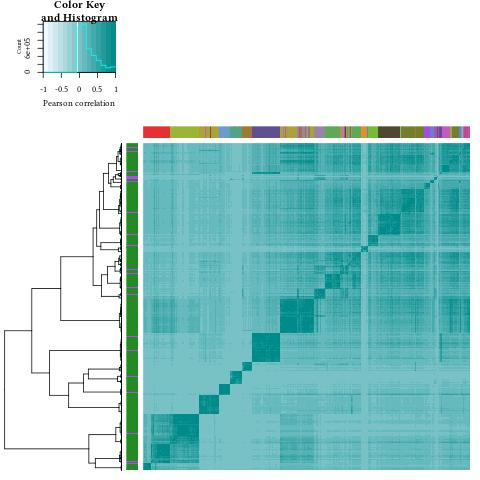
\includegraphics[scale=0.95]{transcriptomics/heatmap23Replicates.jpg}\centering
    \caption[Heatmap including all the replicates of the 23 common tissues
    between Uhlén and GTEx studies]{\label{fig:noMitoRep23T}\textbf{Heatmap
    including all the replicates of the 23 common tissues between \uhlen\ and
    \gtex\ studies.} All protein coding genes (except the mitochondrial ones)
    at least expressed at 1 \FPKM\ are included. Most samples are clustering by
    their tissue of origin while we can observe than many single replicates may
    cluster less expectedly. Many small mixtures are observed, often they involve
    closely related tissues, \ie\ \tissue{Heart} and \tissue{Skeletal muscle} or
    \tissue{Ovary} and \tissue{Fallopian tube}.}
\end{figure}

\begin{figure}[htpb]
\includegraphics[scale=1]{transcriptomics/highExpress4TP.pdf}\centering
\caption[Cumulative shared set of genes ranked by expression across the 5
studies]{\label{fig:highExpress4T}\textbf{Cumulative shared set of genes
ranked by their decreasing order of expression across the 5 studies.}
Except a very small subset for the highest expressed protein coding genes,
the overlap of the gene ranks across the 5 studies is rather small.
The grey line presents the evolution of the ratios for the randomly
permuted data which highlights that there is an underlying structure.}
\end{figure}

\begin{figure}[htpb]
    \includegraphics[scale=1]{transcriptomics/highExpress23TP.pdf}\centering
    \caption[Cumulative shared set of genes, sorted by their expression, between
    Uhlen and GTEx]{\label{fig:highExpress23T}\textbf{Cumulative shared set of
    genes, ranked by their decreasing order of expression, between \uhlen\ and
    \gtex\ studies.}
    The highest expressed genes present greater ratios than
    when the 5 studies are considered (see \Cref{fig:highExpress4T}).
    The fewer number of studies considered, which, additionally to be the most
    recent studies, are the ones to comprise greater number of biological
    replicates per tissues may be the sole reasons for the improved results.}
\end{figure}

\begin{figure}[htpb]
\centering
\begin{minipage}{\textwidth}
\begin{subfigure}[b]{0.95\textwidth}
\centering
\includegraphics[scale=0.9]%
{transcriptomics/TransPearsonDistributionIdenticalDifferent.pdf}
\caption[Pearson correlation]{\label{fig:distribPearsCorr}\textbf{Pearson
correlation}}
\end{subfigure}

\begin{subfigure}[b]{0.95\textwidth}
\centering
\includegraphics[scale=0.9]%
{transcriptomics/TransSpearmanDistributionIdenticalDifferent.pdf}
\caption[Spearman correlation]{\label{fig:distribSpearCorr}\textbf{Spearman
correlation}}
\end{subfigure}
\caption[Distribution of the correlation of matched and unmatched tissues pairs
across the two working sets.]{\label{fig:distribCorr}%
\textbf{Distribution of the correlation of matched
and unmatched tissues pairs for the two working sets.} The displayed
p-values\footnote{Thresholds above which the $H_0$ hypothesis
is safe to be rejected.\\$H_0$: The correlations of same tissue pairs and
different tissues pairs are similar.} have been computed with
a Welch two-sample t-test.}
\end{minipage}
\end{figure}


\begin{sidewaysfigure}[htpb]
    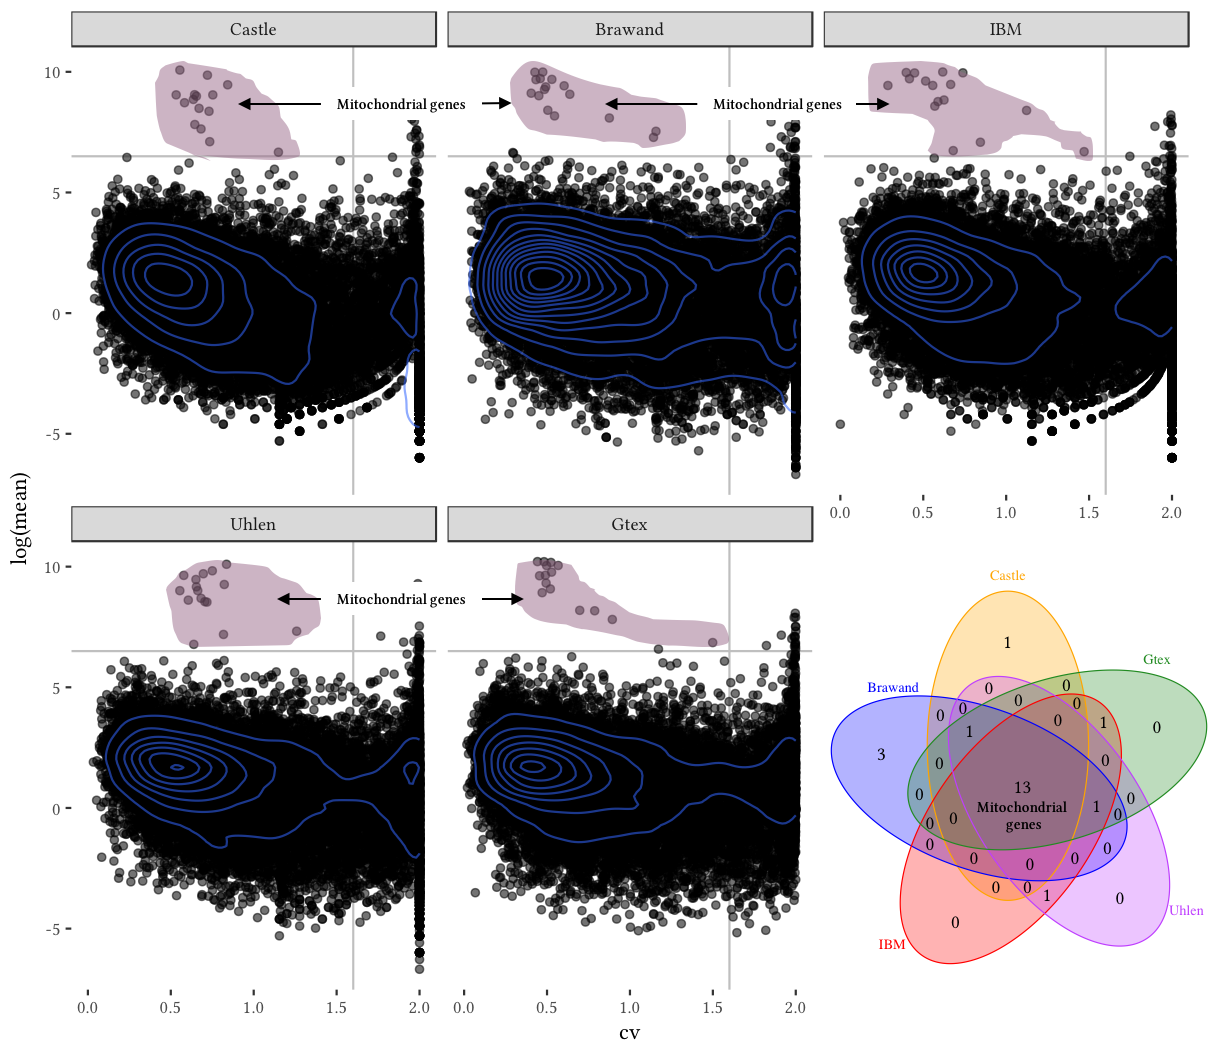
\includegraphics[scale=1]{transcriptomics/MitoVarianceFinale.png}\centering
    \caption[Mean expression of genes compared to their coefficient of variation]%
    {\label{fig:MitoVar}\textbf{Mean expression of genes compared to their
    coefficient of variation.}}
\end{sidewaysfigure}

\begin{figure}[!htpb]
    \includegraphics[scale=0.7]{transcriptomics/Overlap_25p_mostCoeffVariablesgenes.pdf}\centering
    \caption[Overlap of the most variables genes across the 5 studies for the set
    of four common tissues]{\label{fig:vennMostVar4T}\textbf{Overlap of the most
    variable genes across the 5 studies for the set of the four common tissues.}
    In each study, I rank the \pcgs\ in decreasing order.
    This Venn diagram presents the shared and unique \pcgs\ in the top
    quarter of the most variable genes.
    }
\end{figure}

\minisec{Two-sample test}\label{mini:ttest}
\TK{Explain Welch, Student}
The Welch test,
also known as the unequal variances \ttest,
is an adaptation of the Student \ttest.
Except in case of (true) paired data (sampled on the same source),
it gives better or at least equal results than the traditional Student \ttest.

\begin{figure}[!htpb]
    \includegraphics[scale=0.90]%
    {transcriptomics/Heatmap_25p_mostCoeffVariablesgenes_spearman.pdf}\centering
    \caption[Clustering of the four common tissues across the five studies for
    the most common variable genes]%
    {\label{fig:heatmapMost25pVariable}\textbf{Clustering of the four common
    tissues across the five studies for the most common variable genes.}
    The samples cluster by tissue of origin
    rather than by original study.
    Each cluster of tissue presents a different hierarchy of study:
    for \kidney, \uhlen\ sample is closer to the \ibm\ sample,
    while for \testis, \uhlen\ sample is closer to the \gtex\ one.}
\end{figure}

\begin{figure}[!htpb]
    \includegraphics[scale=0.90]%
    {transcriptomics/Reverse_heatmap_25p_mostCoeffVariablesgenes_Spearman.pdf}\centering
    \caption[Clustering of the the four common tissues across the five studies
    (excluding the most common variable genes)]{\label{fig:ReverseheatmapMost25pVariable}%
    \textbf{Clustering of the four common tissues across the five studies
    (excluding the most variable genes).} Except the Castle samples,
    the samples cluster by tissue of origin rather than by original study.
    (Note that Pearson correlations give more results.)}
\end{figure}

\begin{figure}[!htpb]
    \includegraphics[scale=0.8]{transcriptomics/Heatmap_25p_mostCoeffVariablesgenesTheirExpression.pdf}\centering
    \caption[Expression of the most common variable genes]{\label{fig:expressionMostvariableG}
    \textbf{Expression of the most common variable genes.} }
\end{figure}

\begin{comment}
\begin{figure}[htpb]
    \includegraphics[scale=1]{transcriptomics/mostSpe23TP.pdf}\centering
    \caption[Cumulative shared set of genes, sorted by their specificity, between
Uhlen and GTEx]{\label{fig:mostSpe23T}\textbf{Cumulative shared set of genes
ordered by their decreasing order of specificity to each tissue between \uhlen\
and \gtex.}}
\end{figure}
\end{comment}

\section{Hampel method}

\begin{algorithm}[H]
\SetAlgoLined
\KwData{Expression matrix; Genes as rows and conditions as columns}
\KwResult{Indicates if a gene presents an \emph{outlier} expression for any condition
(as a boolean or a numeric ratio)}
\BlankLine\
\While{not at end of this document}{
read current\;
\eIf{understand}{
go to next section\;
current section becomes this one\;
}{
go back to the beginning of current section\;
}
}
\caption{Hampel method}\label{algo:hampel}
\end{algorithm}

\begin{algorithm}[H]
\SetAlgoLined
\KwData{Numerical vector $v$}
\KwResult{\gls{MAD} of the vector $v$}

\caption{Median absolute deviation (MAD)}\label{algo:mad}
\end{algorithm}



\begin{comment}
\begin{algorithm}[H]
\SetAlgoLined\
\KwData{\KwResult{}
\Input{An expression matrix $m$}
\Output{A boolean or numeric matrix $mo$}
\BlankLine\
\lForEach{gene $g$ of the matrix $m$}{\\
   $median \leftarrow\ computeMedian(g)$\;
   $MAD \leftarrow\ computeMAD(g)$\;}

\caption{\end{algorithm}
\end{comment}

\section{List of the tissues available in TiGER}\label{sec:supplTiger}

Thirty tissues (or equivalent) are available through this database:
\tissue{Bladder}, \tissue{blood}, \tissue{Bone}, \tissue{Bone marrow},
\tissue{Brain}, \tissue{Cervix}, \tissue{Colon}, \tissue{Eye},
\tissue{Heart}, \tissue{Kidney}, \tissue{Larynx}, \tissue{Liver},
\tissue{Lung}, \tissue{Lymph node}, \tissue{Mammary gland}, \tissue{Muscle},
\tissue{Ovary}, \tissue{Pancreas}, \tissue{Peripheral nervous system},
\tissue{Placenta}, \tissue{Prostate}, \tissue{Skin},
\tissue{Small intestine}, \tissue{Soft tissue}, \tissue{Spleen},
\tissue{Stomach}, \tissue{Testis}, \tissue{Thymus}, \tissue{Tongue} and \tissue{Uterus}.

\begin{comment}
\begin{sidewaystable}[]
\centering
\caption{My caption}
\label{tab:TiGERperTissue}
\begin{tabular}{@{}cccccccccccccccccc@{}}
\toprule
 & Bladder & Brain & Colon & Heart & Kidney & Liver & Lung & Muscle & Ovary &
 Pancreas & Prostate & Skin &
 \begin{tabular}[c]{@{}c@{}}Small\\ intestine\end{tabular}
 & Spleen & Stomach & Testis & Uterus \\
\midrule
Bladder & 138 & 0 & 4 & 2 & 1 & 6 & 1 & 0 & 0 & 0 & 1 & 3 & 1 & 7 & 1 & 6 & 0 \\
Brain & 0 & 282 & 0 & 0 & 0 & 0 & 0 & 0 & 0 & 0 & 0 & 0 & 0 & 0 & 0 & 0 & 0 \\
Colon & 4 & 0 & 154 & 1 & 12 & 3 & 1 & 0 & 1 & 2 & 1 & 1 & 5 & 1 & 12 & 0 & 0 \\
Heart & 2 & 0 & 1 & 167 & 6 & 1 & 0 & 40 & 5 & 0 & 2 & 2 & 3 & 5 & 1 & 0 & 0 \\
Kidney & 1 & 0 & 12 & 6 & 314 & 39 & 0 & 4 & 3 & 3 & 5 & 0 & 0 & 2 & 3 & 5 & 0 \\
Liver & 6 & 0 & 3 & 1 & 39 & 285 & 1 & 7 & 0 & 3 & 1 & 2 & 3 & 14 & 5 & 9 & 0 \\
Lung & 1 & 0 & 1 & 0 & 0 & 1 & 114 & 0 & 0 & 3 & 2 & 0 & 0 & 0 & 2 & 1 & 0 \\
Muscle & 0 & 0 & 0 & 40 & 4 & 7 & 0 & 203 & 1 & 1 & 2 & 1 & 5 & 2 & 0 & 1 & 0 \\
Ovary & 0 & 0 & 1 & 5 & 3 & 0 & 0 & 1 & 110 & 1 & 1 & 0 & 1 & 1 & 5 & 2 & 1 \\
Pancreas & 0 & 0 & 2 & 0 & 3 & 3 & 3 & 1 & 1 & 145 & 0 & 1 & 2 & 0 & 8 & 2 & 0 \\
Prostate & 1 & 0 & 1 & 2 & 5 & 1 & 2 & 2 & 1 & 0 & 127 & 2 & 1 & 1 & 1 & 3 & 0 \\
Skin & 3 & 0 & 1 & 2 & 0 & 2 & 0 & 1 & 0 & 1 & 2 & 143 & 0 & 0 & 0 & 2 & 0 \\
\begin{tabular}[c]{@{}c@{}}Small\\ intestine\end{tabular} & 1 & 0 & 5 & 3 & 0 & 3 & 0 & 5 & 1 & 2 & 1 & 0 & 96 & 3 & 1 & 1 & 0 \\
Spleen & 7 & 0 & 1 & 5 & 2 & 14 & 0 & 2 & 1 & 0 & 1 & 0 & 3 & 97 & 8 & 2 & 0 \\
Stomach & 1 & 0 & 12 & 1 & 3 & 5 & 2 & 0 & 5 & 8 & 1 & 0 & 1 & 8 & 174 & 1 & 1 \\
Testis & 6 & 0 & 0 & 0 & 5 & 9 & 1 & 1 & 2 & 2 & 3 & 2 & 1 & 2 & 1 & 636 & 2 \\
Uterus & 0 & 0 & 0 & 0 & 0 & 0 & 0 & 0 & 1 & 0 & 0 & 0 & 0 & 0 & 1 & 2 & 39 \\
\bottomrule
\end{tabular}
\end{sidewaystable}
\end{comment}


\section{Uhlén categories}\label{sec:suppUhlen}

\begin{sidewaystable}[]
\centering
\caption{My caption}
\label{tab:uhlenCatAllgenes}
\begin{tabular}{@{}ccccccccccc@{}}
\toprule
\multicolumn{2}{c}{\multirow{2}{*}{\begin{tabular}[c]{@{}c@{}}\ens{76}
\\(62,757 gene definitions) \end{tabular}}} &
\multirow{2}{*}{\begin{tabular}[c]{@{}c@{}}\\Not\\detected\end{tabular}} &
\multirow{3}{*}{\begin{tabular}[c]{@{}c@{}}Not expressed\\ at 1 \gls{FPKM}\\
    cut-off\end{tabular}} &
\multicolumn{2}{c}{Mixed expression} &
\multicolumn{2}{c}{Ubiquitous expression} &
\multirow{2}{*}{\begin{tabular}[c]{@{}c@{}}\\Group \\Enhanced\end{tabular}} &
\multirow{2}{*}{\begin{tabular}[c]{@{}c@{}}\\Tissue\\ Enhanced\end{tabular}} &
\multirow{2}{*}{\begin{tabular}[c]{@{}c@{}}\\Tissue\\ Enriched\end{tabular}} \\
\cmidrule(lr){5-8}
\multicolumn{2}{c}{}   &  &  &
    \begin{tabular}[c]{@{}c@{}}Low\\ (\textless\ 10 \gls{FPKM})\end{tabular} &
    \begin{tabular}[c]{@{}c@{}}High\\ (≥ 10 \gls{FPKM})\end{tabular} &
    \begin{tabular}[c]{@{}c@{}}Low\\ (\textless\ 10 \gls{FPKM})\end{tabular} &
    \begin{tabular}[c]{@{}c@{}}High\\ (≥ 10 FPKM)\end{tabular} &  &  &  \\
\midrule
\multicolumn{1}{c}{%
    \multirow{7}{*}{\rotatebox[origin=c]{90}{\parbox[c]{4cm}{\centering Whole
     dataset}}}} &
     Castle & 18,836 & 16,258 & 19,079 & 1,203  &
     1,456  & 703  & 77  & 8,319  & 3,896 \\
     \multicolumn{1}{c}{} & Brawand & 18,278 & 20,173 &
     15,254 & 2,057  & 1,873 & 977   & 0  &
     6,180  & 5,442 \\
     \multicolumn{1}{c}{} & IBM & 14,494 & 20,858  &
     16,633  & 1,582  & 1,194 & 926  & 733 &
     10,042  & 4,453  \\
     \multicolumn{1}{c}{} & Uhlen & 17,345 & 16,548 &
     15,372 & 1,351  & 467 & 419  & 4,615  &
     10,644 & 5,498  \\
     \multicolumn{1}{c}{} & Gtex  & 5,755  & 25,138  &
     17,172  & 1,464 & 775  & 713  & 7,164  &
     10,032  & 5,117 \\ \cmidrule(l){2-11}
     \multicolumn{1}{c}{} & Consensus & 5,747 & 4,231  &
     4,121  & 230  & 33  & 166  & 0  & 1,073  &
     \begin{tabular}[c]{@{}c@{}}531 $[$518$]$\end{tabular} \\
\midrule
\multirow{7}{*}{\rotatebox[origin=c]{90}{\parbox[c]{3cm}{\centering Common\\
4 tissues\\ Working datasets}}} &
Castle & 43,921 & 3,267 & 14,850 & 1,735 &
3,267 & 1,181 & --- & --- & 4,645 \\
& Brawand & 44,479  & 3,193  & 13,975 & 2,541
& 3,193  & 1,282 & --- & --- & 7,002  \\
& IBM & 48,263  & 3,262 & 13,672 & 2,160 &
3,262  & 1,299  & --- & --- & 5,242  \\
& Uhlen & 45,412 & 3,146 & 14,332 & 2,546 &
3,146 & 1,213  & --- & --- & 7,665  \\
& Gtex & 57,002 & 4,516 & 16,652  & 2,771 &
4,516  & 1,459  & --- & --- & 8,155  \\
\cmidrule(l){2-11}
& Consensus & 9,655 & 557 & 4,366 & 675 &
557  & 448 & --- & --- & 1,960  \\
\\ \midrule
\multirow{3}{*}{\rotatebox[origin=c]{90}{\parbox[c]{1.7cm}{\centering Common\\ 23
tissues\\ Working datasets}}} & Uhlen & 17,345  & 27,575  &
14,981 & 1,427 & 611  & 440 & 2,203 & 11,252 & 5,678 \\
& Gtex & 5,755 & 38,988 & 16,982  & 1,909 & 2,122  & 1,021 & 1,746 & 11,236
& 5,971 \\
\cmidrule(l){2-11}
& Consensus & 5,755 & 27,149 & 12,250 & 973 &
433 & 430 & 797 & 8,030 & 4,281 \\
\bottomrule
\end{tabular}
\end{sidewaystable}


